\documentclass{article}
\usepackage{tikz}
\usetikzlibrary {angles, quotes}

\begin{document}

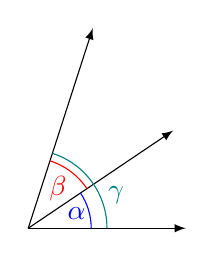
\begin{tikzpicture}
             
\coordinate (o) at (0,0);
\coordinate (u) at (1.84,1.24);
\coordinate (v) at (0.82,2.54);
\coordinate (x) at (2,0);

\draw [-latex] (o) -- (u);
\draw [-latex] (o) -- (v);
\draw [-latex] (o) -- (x);

\path pic[draw=blue, angle radius=8mm, "$\alpha$", blue, angle eccentricity=.8]{angle=x--o--u};
\path pic[draw=red, angle radius=9mm, "$\beta$", red, angle eccentricity=.7]{angle=u--o--v};
\path pic[draw=teal, angle radius=10mm, "$\gamma$", below right, teal, angle eccentricity=1.1]{angle=x--o--v};

\end{tikzpicture}

\end{document}